\documentclass[a4paper,top=25mm,bottom=25mm,12pt,pdftex,halfparskip,twoside,bibtotoc,numbers=noenddot]{scrbook}

\raggedbottom

\usepackage{fancyhdr}

\usepackage[utf8]{inputenc}
\usepackage{wrapfig}
\usepackage[pdftex]{graphicx}
\usepackage{caption}
\usepackage{subcaption}
\usepackage{eso-pic}
\usepackage{array}
\usepackage{pgfplots}
\usepackage{tabularx}
\usepackage{makecell}
\usepackage{multicol}
\usepackage{xcolor}
\usepackage{float}
\usepackage{enumitem}
\usepackage{listings}
\usepackage[toc,page]{appendix}
\usepackage[english]{babel}
\usepackage[backend=biber, style=numeric, natbib=true, hyperref=true]{biblatex}

\addbibresource{thesis.bib}

\linespread{1.25}

% chapters, numbering
\newcommand{\xchapter}{\stepcounter{chapter}\setcounter{section}{0}\addchap}

% tables
\renewcommand\theadalign{bc}
\renewcommand\theadfont{\bfseries}
%\renewcommand\theadgape{\Gape[4pt]}
\renewcommand\cellgape{\Gape[1pt]}
\renewcommand{\arraystretch}{2.5}
\setlength{\tabcolsep}{4pt}

\graphicspath{{img/}}

\fancypagestyle{plain}{%
	\fancyhf{}%
	\fancyfoot[LO,RE]{\thepage}%
	\renewcommand{\headrulewidth}{0pt}
}

\definecolor{gray}{rgb}{0.4,0.4,0.4}
\definecolor{darkblue}{rgb}{0.0,0.0,0.6}
\definecolor{cyan}{rgb}{0.0,0.6,0.6}
\definecolor{green}{rgb}{0,0.6,0}
\definecolor{mauve}{rgb}{0.58,0,0.82}

\lstset{
  basicstyle=\ttfamily,
  columns=fullflexible,
  showstringspaces=false,
  captionpos=b,
  commentstyle=\color{gray}\upshape,
  keywordstyle=\color{blue},       % keyword style
  stringstyle=\color{mauve},
}

\lstdefinelanguage{XML}
{
  morestring=[b]",
  morestring=[s]{>}{<},
  morecomment=[s]{<?}{?>},
  stringstyle=\color{black},
  identifierstyle=\color{darkblue},
  keywordstyle=\color{cyan},
  morekeywords={xmlns,version,type,name,as,id,style,x,y,width,height}% list your attributes here
}

% define medatata
\def\MOrg{Leopold-Franzens-University Innsbruck}
\def\MInstitution{Department of Computer Science}
\def\MGroup{Distributed and Parallel Systems Group}
\def\MTitle{High-Level Modeling and Low-Level Adaptation of Serverless Function Choreographies}
\def\MAuthor{Benjamin Walch\\ \small 01518922}
\def\MSupervisor{Shashko Ristov, PhD}
\def\MDate{\today}

\begin{document}

\frontmatter
\pagestyle{empty}

\begin{titlepage}
\rule{0mm}{1mm}

\begin{multicols}{2}[\columnsep2em] 
	\includegraphics[width=6cm]{uibk-logo}
	\columnbreak
	\begin{flushright}
		\Large{\textsf{\MOrg}}
	\end{flushright}
\end{multicols}

\begin{flushright}
	{\large \MInstitution\\}
	{\large \MGroup}
\end{flushright}

\vspace*{1.5cm}

\begin{center}
	{\LARGE\bf \MTitle}
	\vskip 2.25cm
	\Large \textbf{Bachelor Thesis}
	\vskip 2.25cm
	{\Large \MAuthor}
	\vskip 1.5cm
	{\large Supervisor: \MSupervisor}   
	\vfill
	{\large Innsbruck, \MDate}
\end{center}
\AddToShipoutPicture{
	\put(-55,55){
		\parbox[b]{\paperwidth}{
			\hfill \includegraphics[scale=0.35]{uibk-watermark}
		}
	}
}
\end{titlepage} 

\ClearShipoutPicture

\clearpage

\section*{Declaration}

By  my  own  signature  I  declare  that  I  produced  this  work  as  the  sole author, working independently, and that I did not use any sources and aids other than those referenced in the text. All passages borrowed from external sources, verbatim or by content, are explicitly identified as such.

I consent to the archiving of the bachelor thesis at the institute / faculty:

\vspace{1.8cm}

\parbox{6cm}{
	\hrule
	\strut \centering\footnotesize Date
} \hfill
\parbox{6cm}{
	\hrule
	\strut \centering\footnotesize Signature
}

\clearpage

\thispagestyle{plain}

\vspace{2.5cm}
\begin{center}
\textbf{Abstract}
\end{center}

% to be written at the end!
% some results ..

The Distributed and Parallel Systems group developed the \emph{Abstract Function Choreography Language} (AFCL). It is a specification for describing serverless workflows. Furthermore, a Java API, to describe serverless application workflows programmatically, was developed.
The product which results in using that API is a workflow being described in AFCL in a text based file.
Until now, the workflow being described in the text file has to be created manually (by editing the file directly), or a programmer has to write Java code which utilizes the API to generate the file.
\par
The aim of this bachelor project is to develop a visual workflow editor, which makes modeling of workflows possible at a high level of abstraction. The tool should not only be able to load, display and save workflows, but also optimize workflows for multiple FaaS provider(s) in case of quotas and limits, and also in case of performance.

\tableofcontents

\listoffigures

\listoftables

\mainmatter
\pagestyle{fancy}

\renewcommand{\chaptermark}[1]{%
	\markboth{\thechapter.\ #1}{}
}

\fancyhead{}
\fancyhead[LO]{\leftmark}
\fancyhead[RE]{\rightmark}
\fancyfoot{}
\fancyfoot[LO,RE]{\thepage}

\label{chap:introduction}
\chapter{Introduction}

% - Why is the work important?
% - provider specific implementations
% - need tool to create easily 


% In the FaaS world, there exist many providers who offer serverless execution of code (functions) in the cloud. Each of them has its own specifications and definitions on how functions are deployed and executed, and how workflows are created and executed.
"Run code, not Servers" is a recent term in the cloud computing world.
With the rise of serverless technologies during the last years, \emph{Function-as-a-Service} (FaaS) became more and more popular. This cloud computing concept offers new advantages for software development: very high flexibility, nearly unlimited scalability and pay-per-use pricing. Entire programs can be defined in workflows and can be executed using serverless technology in the cloud.

However, each serverless provider has its own definitions on how a workflow is expressed, as well as different pricing models, limits and quotas. For example, the maximum number of concurrent function invocations is limited to 1000 concurrent invocations for current FaaS providers at time of writing.\footnote{checked providers: AWS, Google, IBM and Microsoft}
In addition, different providers also support different programming languages. That being said, a workflow from one system is not compatible with another, what means, the user is bound to a specific provider (vendor lock-in), if the workflow is considered to be reused.

Many FaaS providers offer tools which should support and simplify creation of workflows in their environment. Nevertheless, this is still a complex task. Most of the time, a software developer is needed, because others simply lack the neccessary know-how; and even for developers, this task can be tedious and time-consuming.

The distributed and parallel systems group developed a specification to describe serverless workflows at a high abstraction level. This specification is called \emph{Abstract Function Choreography Language} (AFCL) and was created to overcome weaknesses  of current FaaS platforms; for example incompatibility of workflows between different providers, which would make also cross-cloud workflow execution possible.

Castro et al. mentions that "One of the major challenges slowing the adoption of serverless is the lack of tools and frameworks" \cite{articles-rise-of-serverless-castro}.\\
Therefore, the goal for this thesis is to implement a new tool providing a system, able to create AFCL workflows at a high level of abstraction. In addition, visualizing - in particular loading, displaying and editing - of existing AFCL workflows in should be supported.
The system should also provide an interface for performing workflow adaptations at low-level, based on specific inputs.

This thesis fulfills above goals and overcomes mentioned problems.
With the developed system, which we call "AFCL ToolKit" in the further text, it is possible for non-developers to create a workflow in less time than it would have taken a developer to write the workflow in AFCL.\\
Another advantage is that workflows created with AFCL ToolKit are guaranteed to be valid AFCL, which minimizes the rate of human errors.

Regarding provider limitations, a scheduler (which is not part of this thesis) would decide to distribute for example one big concurrent loop - with more iterations than the maximum number of function invocations allowed by the provider - onto multiple FaaS providers. For this purpose, a service is provided which offers an interface for specific workflow adaptations.

% with the GUI it is easier to use the API, such that non-developers can develop an application which is compliant with the API.
% optimization: goal of scheduler is to convert AFCL to CFCL based on the decision which function is executed where. an interface is offered such that the scheduler. Regarding limits of each provider, the scheduler should adapt the workflow to distribute on big loop in multiple providers. For this purpose, we will provide a service, which offers this low-level adaptation.

It is assumed that concrete implementations of the functions are already developed and deployed to a FaaS provider.

In the next chapter, we will give background information to topics related to this thesis. After that, we will look closer at the implementation af AFCL ToolKit, in particular the system architecture and design, before the application's interface is presented and explained. 

After that, we evaluate AFCL ToolKit, which clarifies the benefit of the developed system.

%After that 

\label{chap:background}
\chapter{Background}

This chapter contains important details on the terms and technologies used in this thesis and helps the reader to better understand the further topics.\\
First of all, the serverless concept, in particular Function-as-a-Service, Serverless Functions and Workflows are explained, before giving a brief overview about AFCL. The tools and technologies used for development are also presented to readers who are not yet familiar with them.

\section{Serverless Computing}

Serverless computing is widely known as an event-driven cloud execution model.
In this model, the client provides the code  and the cloud provider manages the life-cycle of the execution environment of that code.
The idea is based on reducing the life span of the program to execute functionality in response to an event. Hence, the program's processes are born when an event is triggered and are killed after the event is processed \cite{inproceedings-serverless-beyond-the-cloud-kanso}.
Developers can completely focus on the program they need to run and not worry at all about the machine it is on or the resources it requires \cite{articles-going-serverless-savage}.
Castro et al. define serverless computing as follows: "Serverless computing is a platform that hides server usage from developers and runs code on-demand automatically scaled and billed only for the time the code is running" \cite{articles-rise-of-serverless-castro}.

The term "serverless" can be misleading though, as there are still servers providing these backend services, but all of the server space and infrastructure concerns are handled by the vendor. Serverless means that the developers can do their work without having to worry about servers at all \cite{online-what-is-serverless-cloudflare}.

\section{FaaS}

FaaS is a form of serverless computing, which is disrupting the way applications and systems have been built for decades. By abstracting infrastructure provisioning and deployment, user-provided functions can be invoked and executed remotely. The user only has to worry about development and triggering of the function. This serverless runtime has not only the advantage that it avoids costly pre-allocated or dedicated hardware, but also offers almost unlimited possibilities in scalability. FaaS systems are designed to allow a usage-based billing, what means the user will only be charged for resources required during execution.

\section{Serverless Functions}
Serverless functions - or tasks - are single-purpose, mostly stateless, programmatic functions that are hosted on cloud infrastructure. These infrastructure is provided through a FaaS platform. They are event-driven and can be invoked through the internet, mainly using HTTP. Like conventional functions, they accept arguments and and return the result of the computation  - with the difference that this is done over a network.

\section{Serverless Workflows}
On an abstract level, a workflow consists of a set of interdependent tasks that need to be executed to achieve a specific goal. [...] A task within a workflow has the following properties: dependencies on the software or service used by the task to perform its computation (software flow), dependencies on data (data flow), and dependencies on other tasks (control flow) \cite{thesis-design-serverless-worfklow-system-eyk}.\\
Basic and advanced control flow patterns for workflows are shown in \cite{reports-workflow-control-patterns-russell}.

A serverless workflow is a complex workflow defined through the composition of serverless functions, connected by control- and data flow. Serverless workflows make it possible to combine and reuse serverless functions in order to build more complex applications. 
Workflows can declare the structure of applications - and using formats like YAML, XML or JSON, they can be described in a text-based file.

\section{AFCL}

This section gives the reader a brief overview on AFCL and its features. More detailed information about AFCL as well as the API documentation can be found at \cite{online-afcl-dps}.

The \emph{Abstract Function Choreography Language} (AFCL) was created to overcome weaknesses in current FaaS platform implementations. As the name indicates, this specification describes serverless workflows at a high level of abstraction, forming a step on the way to cross-cloud workflow execution.\\
Consider a workflow built with AWS Step Functions, should be executed on IBM Cloud. To make that work, the workflow has to be ported to the other platform to be compatible. In other words - it has to be recreated by a skilled programmer - for example by using the exported workflow as a template.

The AFCL specification also has more extensive control-flow and data-flow constructs available than current FaaS providers offer currently in terms of language features. Therefore, AFCL can not only eliminate the incompatibility of workflows between different providers (vendor lock-in), but also opens the door to execute a workflow by distributing its computation over multiple FaaS providers.

To be able to actually execute such multi-cloud workflows, some more tools are needed: an Enactment Engine and a Scheduler.

\subsection{Overview}
% here the different control structures of AFCL?
AFCL is based on YAML\footnote{https://yaml.org} and ships with a schema\footnote{http://dps.uibk.ac.at/projects/afcl/files/schema/schema.yaml}. There exist two types of functions, base functions and compound functions, which can be connected by specifying control-flow and data-flow information. While base functions represent a single task, compound functions provide nesting - they can include some base functions or even other compound functions.

Base and compound functions have data input (dataIns) and data output (dataOuts) ports to define input or output data, respectively.
Data input can refer to another data output or data input of another function by specifying the name in combination with the data ouput port of the other function.

\subsection{Control-flow}
In AFCL, base or compound functions are specified one after another, which means that they are executed sequential. However, the following control constructs are introduced with AFCL: \texttt{sequence}, \texttt{if-then-else}, \texttt{switch}, \texttt{for}, \texttt{while}, \texttt{parallel} and \texttt{parallelFor}.


\subsection{Properties and Constraints}

Additional, optional attributes for \texttt{dataIns} and \texttt{dataOuts} ports of a function, or for the function itself can be defined in \texttt{properties} and \texttt{constraints}. While those are simple key-value pairs accepting string values, AFCL has a few defined properties and constraints to specify concrete attributes like invocation type of a function, element index or data distribution information in loops.

% data flow (dag based)
\subsection{Data-flow}
AFCL allows to express data-flow by connecting source data ports of functions to target data ports of functions. This offers support for more complex data-flow scenarios and might improve performance of the workflow. A source data port can be the input data port of the whole workflow, or a data port (input or output) of another function. So it is possible to even connect data ports of outer functions with a a lower nesting level to inner functions with a higher nesting level. 

\section{Tools and Technologies}
\subsection{npm}

The \textit{node package manager} is the world's largest software registry, where open-source software packages of developers and companies are shared all over the world.\footnote{https://www.npmjs.org} Over the last years, \textit{npm} became a de-facto standard for package management in JavaScript development.

\subsection{webpack}

\textit{webpack} is a module bundler, its main purpose is to bundle JavaScript code for the usage in a browser.\footnote{https://webpack.js.org} In particular, multiple modules (often hundreds of) with dependencies [to each other] are processed and bundled into a few files. To be able to process other types of files than JavaScript or JSON, webpack offers the opportunity to configure a \textbf{loader}. In this application, the following loaders are configured:
\begin{itemize}
\item babel-loader, to transform ES and React JSX to browser-compatible JavaScript
\item sass-loader, to transform SASS to CSS
\item css-loader, to transform CSS to CommonJS
\item file-loader, to handle static resources like images and fonts
\end{itemize}

\subsection{ECMAScript}

The scripting language specification \textit{ECMAScript} (ES) was created to standardize JavaScript. With the release of ES6 (also known as ECMAScript 2015), features like class declarations, module imports and arrow function expressions became possible. After ES6, every year a new edition of the ECMAScript standard was finalized and released, offering new features. Worth mentioning here is the rest/spread operator released with ES9, which was used a lot in this thesis.

\subsection{Babel}
Since current browsers only have partial support of ECMAScript, a \textit{transcompiler} or \textit{transpiler} is needed to transform the ECMAScript source code to JavaScript, which common browsers are capable of interpreting.
\textit{Babel} is an industry standard to transpile ES to common JavaScript or lower ES versions.\footnote{https://babeljs.io}

\subsection{SASS}

CSS, in its pure form, reaches its limits when one thinks about using variables, functions or nested rules. \textit{SASS} is a stylesheet language, which is\footnote{https://sass-lang.com} - similiar to ES - compiled to CSS and offers the mentioned and even more features.
A lot of CSS Frameworks also provide their source code in SASS, often served with a large variable set which makes customization easy.

\chapter{AFCL ToolKit}

This chapter gives the reader a detailed overview over the system architecture and the system design, including evaluations for technology decicions for specific tasks.

AFCL ToolKit should not only visualize AFCL Workflows, but also give non-developers the opportunity to create and edit workflows through a Graphical User Interface (GUI). This GUI ships with a powerful editor, including additional features like real-time validation, change history (versioning), clipboard (copy-paste) and automatic layouting.\\
Furthermore, workflows can be adapted at low-level in order to divide large parallel loops - for example loops with more iterations than allowed by current providers - into several loops which run in parallel. By doing this, AFCL ToolKit also adapts  all existing data flow to respect the new structure.

\section{System Architecture}
% what was built

% show interfaces between modules
% Input output in each
% communication
% (to subsystems: FE constists of this ..., BE constists of this - goals of both BE and FE)
% more grained visualization

% optional 

AFCL ToolKit is built on top of two sub systems which are operating mostly decoupled from each other. On the one hand there is the backend, responsible for low-level operations persistence of function data.\\
On the other hand is the frontend with the GUI, responsible for user interaction, data visualization and file I/O.\\
Those two sub systems interact with each other by sharing JSON-serialized objects through an API the backend provides and the frontend consumes.

% put scheduler on the left side in this graphic
% dashed lines / transparency interface for later

% scheduler has interface
\begin{figure}[H]
  \centering
  \vspace{0.8cm}
  \includegraphics{architecture}
  \caption{system architecture}
\end{figure}

\subsection{Frontend}

% none of serverless impl offers graphical workflow modeling, only visualizing is supported

% explain user's actions, how the system works ...

The frontend displays and controls the application's user interface. Its core component is the workflow editor, which is responsible for visualizing workflow data and provides a drawing area, allowing the user to compose and edit workflows in WYSIWYG manner.\footnote{https://en.wikipedia.org/wiki/WYSIWYG}

The editor allows the user to load, create, edit and save AFCL workflows (YAML or JSON), which visualizes the current workflow as a graph. While editing, actions are constantly validated to a set of constraints which ensures workflows validity. The editor includes an action history which enables undo and redo, as well as a clipboard for copy and paste.

All features of the web-based user interface are described in detail in section \ref{chap:impl-webinterface}.

% present only functionalities
% create workflow
% load workflow
% validator
% "versioning" (command history for undo/redo)
% automatic layout from empty YAML/JSON

% Frontend - explain 
% accepts YAML/JSON - visualize it - save or export it

% details about frontend
% all "boxes" in frontend , all functionalities
%screenshots for functionalities

\subsection{Backend}

The main purpose of the backend is to perform operations on workflows at low-level. These operations include the conversion of XML data delivered from the frontend, as well as complex workflow modifications.
For the communication with the world outside, the backend includes a web server, which is used to expose the endpoint for its HTTP-based API to clients. Moreover, the frontend web application is also delivered by this web server. 
Last but not least, the persisting of function data is also covered by the backend.

% interface for adaptation during runtime such that based on the decision of the scheduler also automatic display of new "optimized" workflow

% all this should be visible on the architecture

% which functional components does the system have!

\section{System Design}

% after overall system was presented, we willl now look deeper into system design
% again present frontend and backend
After the overall system architecture was presented, we will now look deeper into the system design.
This  section  focuses on how the implementation of the system was done.

\subsection{Frontend}
The frontend is built as a web application with HTML, CSS and JavaScript.

The base forms npm, which is used to manage and resolve dependencies.  Webpack is the main part which orchestrates transpiling and bundling all sources and assets into single files by utilizing so-called loaders.

Babel is used as such a webpack loader for transpiling the ECMAScript and React JSX source code to browser-compatible JavaScript.
The same applies for the CSS extension SASS, which is also integrated with a loader, and is used to make the process of styling the user interface more efficient.

webpack also executes some optimization plugins when building for production, which minimizes the size of the final bundle.

\begin{figure}[H]
  \centering
  \vspace{0.8cm}
  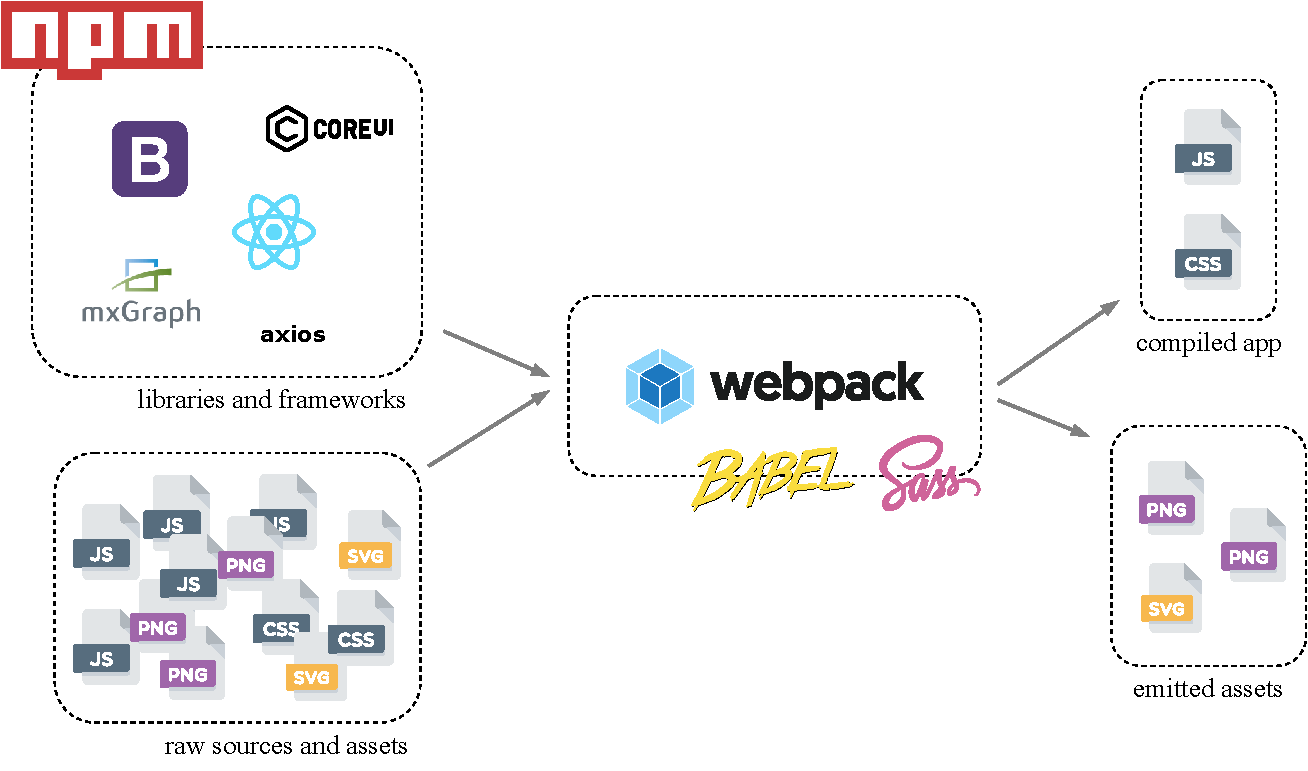
\includegraphics[width=0.8\textwidth]{frontend-setup}
  \caption{frontend stack}
\end{figure}

\subsubsection{Libraries}
Below is a list of selected libraries in this project. Care has been taken to ensure that all libraries used are open source.
\begin{itemize}
\item \textbf{React}\\
React is an JavaScript library for building user interfaces.\footnote{https://reactjs.org}
\item \textbf{mxGraph}\\
mxGraph is a JavaScript diagramming library.\footnote{https://jgraph.github.io/.mxgraph/}
\item \textbf{axios}\\
Axios is a JavaScript library providing a promise based HTTP client for networking tasks.\footnote{https://github.com/axios/axios/}
\item \textbf{Bootstrap}\\
Bootstrap is a toolkit for building web applications.\footnote{https://getbootstrap.com/}.
\item \textbf{CoreUI}\\
CoreUI is a free admin panel template, based on bootstrap.\footnote{https://coreui.io/}
\end{itemize}

\subsubsection{Core Application}

The core application is divided into multiple modules, where each of them was designed to respect the single responsibility principle.\footnote{https://en.wikipedia.org/wiki/Single\_responsibility\_principle} A clean and nested structure of React components forms the user interface of the core  application. One of the benefits when using React is that the data model displayed to the user maps most of the time nicely to UI components.

\subsubsection{Connection to the Backend}

\textit{axios} is used to communicate with the backend, by sending HTTP requests to the corresponding backend endpoint. Data which is sent in the HTTP body, is serialized using JSON, which JavaScript supports out-of-the-box.

\subsubsection{Data model}

All AFCL Java model classes have been ported to ECMAScript, to have all classes and properties available in the frontend, similiar like they are in the backend. Although plain JavaScript objects would also do the job, this adds a kind of type-safety to the ECMAScript sources and improves readability of the code. Also, the data exchange with the backend and the encoding of the graph benefit from this approach, since the XML node names map to constructor names.

\subsubsection{Graph drawing}

A workflow can be represented as a directed acyclic graph (DAG). DAG's are conventional models to present workflows, where nodes are tasks and edges are communications between tasks.

At the time of implementation, the JavaScript library mxGraph was the best choice for the graph visualization and modification.\footnote{see \ref{sec:graph-alternatives} to learn why}
It has an outstanding documentation, enriched with a lot of demos and example code which show many use cases and extensive features, as well as a powerful production-grade example.\footnote{https://draw.io}\\
The authors of mxGraph state:\\
\begin{quote}
``mxGraph is pretty much feature complete, production tested in many large enterprises and stable for many years. We actively fix bugs and add features [...].''
\end{quote}

\subsubsection{Graph model}

In mxGraph, vertices and edges are represented by an \texttt{mxCell} model, which stores information about the position, dimension, geometry and style of the visual element. The \texttt{mxCell} class has been subclassed in a custom class \texttt{Cell}, in order to add user defined logic and an additional \texttt{type} property.

\begin{figure}[H]
  \centering
  \vspace{0.8cm}
  \includegraphics[]{mxCell}
  \caption{\texttt{mxCell} model}
\end{figure}

In the further text, the term \textit{cell} refers to the visual element (which can be a vertex or an edge) in the graph, which represents always an instance of \texttt{Cell}, respectively.

\subsubsection{Graph context}

% \texttt{mxCell} instances are controlled by the \texttt{mxGraphModel}, its visual representation is rendered by \texttt{mxCellRenderer}

A \textit{user object} can be associated with a \texttt{mxCell} through the \texttt{value} property. User objects give the graph its context, they store the business logic associated with the visual part. \cite{manuals-mxgraph-user-manual} For simple cases, the user object may be a string to display the cell's label. In more complex applications, the user object may be an object and some property of that object will generally be the label that the visual cell displays.\\
In this application, the cell's user objects are instances of the ported AFCL classes, and the function name of the AFCL object is used as the label.

\begin{figure}[H]
  \centering
  \vspace{0.5cm}
  \includegraphics[]{cell-user-objects}
  \caption{A graph showing cells and their associated user objects}
\end{figure}

\newpage

The following table shows the implemented \texttt{Cell} types which are used as visual elements representing a node in the graph. Beside a short description, the type of the associated user object is denoted.

\begin{table}[H]
   \centering
\begin{tabular}{ |c|c|c| } 
\hline
\thead{Cell} & \thead{Description} & \thead{User Object} \\
\hline
\makecell{
\includegraphics[width=32pt,height=32pt]{cell-start} \\ \textsf{Start}}  & Defines the workflow's entry point & \makecell{\texttt{String} \\ \small(for the label)} \\
\hline
\makecell{\includegraphics[width=32pt,height=32pt]{cell-end} \\ \textsf{End}}  & Defines the workflow's termination & \makecell{\texttt{String} \\ \small(for the label)} \\
\hline
\makecell{
\includegraphics[width=52pt,height=28pt]{cell-function} \\ \textsf{Function}}  & An atomic function & \texttt{AtomicFunction} * \\
\hline
\makecell{\includegraphics[width=32pt,height=32pt]{cell-ifthenelse} \\ \textsf{If-Then-Else}}  & A mutual exclusive condition & \texttt{IfThenElse} * \\
\hline
\makecell{
\includegraphics[width=32pt,height=32pt]{cell-switch} \\ \textsf{Switch}}  & A multi condition & \texttt{Switch} * \\
\hline
\makecell{
\includegraphics[width=32pt,height=24pt]{cell-merge} \\ \textsf{Merge}}  & An element for merging previous branches & \makecell{\texttt{null} \\ \small(none)} \\
\hline
\makecell{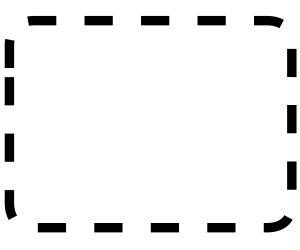
\includegraphics[width=50pt,height=32pt]{cell-compound} \\ \textsf{Parallel}}  & \makecell{A container, where each child cell\\ is meant to be executed in parallel.} & \texttt{Parallel} * \\
\hline
\makecell{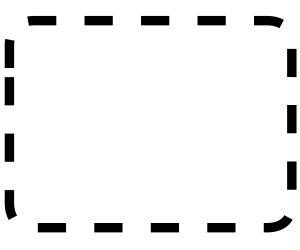
\includegraphics[width=50pt,height=32pt]{cell-compound} \\ \textsf{ParallelFor}}  & \makecell{A container, where each child cell\\ is meant to be executed in a parallel for loop.} & \texttt{ParallelFor} * \\
\hline
\end{tabular}
\caption{Implemented Cells, *: AFCL Object}
\label{tbl:frontend-impl-shapes}
\end{table}

\newpage

\subsubsection{Graph Validation}
\label{sec:impl-frontend-graphvalidation}

A DAG which represents a \textit{valid} AFCL workfow always fulfills the following constraints:

\begin{itemize}
	\item There exists exactly one \textsf{Start}
	\item There exists exactly one \textsf{End}
	\item There exist no cycles
    \item Every \textsf{Cell} has a path to \textsf{Start}
    \item Every \textsf{Cell} has a path to \textsf{End}
	\item \textsf{Function}, \textsf{If-Then-Else}, \textsf{Switch}, \textsf{Parallel}, \textsf{ParallelFor} and \textsf{End} have exactly one incoming edge
	\item \textsf{Start}, \textsf{Function}, \textsf{Parallel}, \textsf{ParallelFor} and \textsf{Merge} have exactly one outgoing edge
	\item \textsf{If-Then-Else} has exactly two outgoing edges (then, else)
	\item \textsf{Switch} has multiple outgoing edges
	\item \textsf{Merge} has multiple incoming edges
\end{itemize}

In addition to the DAG-constraints above, the following additional constraints are needed:

Compound constructs are visualized as container which enclose their child nodes. It has to be ensured that there exists no direct connection from a cell inside a container to a cell outside that container.
\begin{itemize}
	\item Both \textsf{Cell}s taking part in a direct connection, must have the same nesting level, what means they must have the same parent cell
\end{itemize}
In an AFCL workflow, a function's name has to be unique:
\begin{itemize}
	\item A \textsf{Cell}'s label has to be unique in the workflow
\end{itemize}

These constraints are enforced at two different stages: During editing, more specifically when adding and connecting vertices, and before saving or adapting a workflow.
Due the fact that the user cannot even create an invalid workflow in terms of execution flow, efficiency increases and errors in the corresponding backend services will be minimized.


\subsubsection{Graph Encoding}

The visual representation of the workflow and the included data targets human-readability. This data needs to be put into another, proper format for storing. mxGraph provides built-in support for converting the visual representation to XML. An advantage of using XML over JSON is that constructor names (class names) are mapped to the XML node names, no additional property is required.
What makes XML also very convenient is Java's excellent native support for XML and XPath on the backend side. The XML-encoded workflow is converted on backend-side internally to an AFCL workflow.

\begin{lstlisting}[language=XML,caption={Example of a XML-encoded Workflow.},label={lst:xml-workflow-example}]
<Workflow name="Untitled">
  <Array as="dataIns" />
  <Array as="dataOuts" />
  <Array as="body">
    ...
    <Cell id="4" style="fn" type="AtomicFunction" ...>
      <AtomicFunction name="f1" type="f1Type" as="value">
        <Array as="properties" />
        <Array as="constraints" />
        <Array as="dataIns" />
        <Array as="dataOuts" />
      </AtomicFunction>
      <mxGeometry x="40" y="40" width="88" height="32" as="geometry" />
    </Cell>
    ...
  </Array>
</Workflow>
\end{lstlisting}

% example of xml what information is stored 

\subsubsection{Graph Layouting}

When a user loads an AFCL file into the editor, the cells have to be arranged in a way such that the visualization makes sense. There exists no information in AFCL workflows about any visual properties. 

Fortunately, mxGraph ships with multiple layouting algorithms.
For AFCL graphs, the \texttt{mxHierarchicalLayout} algorithm fits best to arrange the elements. This worked pretty well, unless the graph has some container nodes, for which the layouting algorithm broke.
To overcome this problem, a custom layouting algorithm was developed, which layouts all container elements using \texttt{mxHierarchicalLayout} recursively, beginning at the innermost to the outermost container.

\label{sec:graph-alternatives}
\subsubsection{Graph Alternatives}

One of the more difficult tasks was to choose a proper library for graph drawing. Since the graph drawing and visualization is one of the most important features of the frontend, a careful choice has to be made. Of course there exist multiple excellent JavaScript graph drawing libraries, but not all of them are suitable for the requirements of this project.

Below is a list of tested and researched JavaScript graph libraries with additional information why they were insufficient for the project.
\begin{itemize}
	\item \textbf{jsPlumb} is a library of great quality and looks like it would fulfill all  requirements for graph drawing and user interaction out of the box. It has a very good documentation, and a lot of examples. Furthermore its animations and drag and drop handling are outstandingly good. Unfortunately this software is closed-source and a license costs a few thousand dollars.
	\item The same goes for \textbf{Rappid} (formerly known as JointJS) and \textbf{GoJS}, which is even more expensive.
	\item \textbf{diagram-js} is one of the newer diagram libraries. It seems to be a good candidate to draw BPMN graphs.\footnote{http://www.bpmn.org} The lack of an appropriate documentation - even after four years of existence (there exists an open issue on github\footnote{https://github.com/bpmn-io/diagram-js/issues/78} for this) - is still an issue.
	\item \textbf{Cytoscape.js} is older than mxGraph but the development and the community is not less active. This library has a very good documentation and a lot of demos are provided. But it offers fewer examples and "out-of-the-box" features for modeling flowcharts than mxGraph does.
	\item \textbf{vis.js} is a star on npmtrends.\footnote{https://www.npmtrends.com/vis}  It has very smooth animations when manipulating the graph. There exists only one example of graph manipulation on its documentation, it is mainly used for visualization only.
	\item \textbf{Sigma js} is a tiny library with a small documentation. It clearly focuses on displaying and visualizing graphs, not on modeling them. This part would have to be developed manually. Furthermore, the last activity on this project on github was two years ago.
\end{itemize}


\subsection{Backend}

The backend  of the application is built entirely with Java, using Maven as package manager and Apache Tomcat as Servlet Implementation.

\subsubsection{API}
 
The API to interact with the frontend or other clients is based on HTTP and it is inspired by the principles of REST and RPC.

RPC-based APIs are great for actions (that is, procedures or commands).
REST-based APIs are great for modeling your domain (that is, resources or entities), making CRUD (create, read, update, delete) available for all of your data. \cite{online-smashingmagazine-rest-vs-rpc}

Function data is stored on server-side, thus its API is a REST-based implementation. Workflows are stored in files on a user's disk and workflow adaptation is a "remote command" which just sends data to the server and asks it to process and return the result. Therefore the API to adapt workflows is RPC-based. All API requests use JSON as format for receiving and returning data.

\subsubsection{Decoding Frontend Data}
\label{sec:backend-decoding}

Since the frontend encodes its visual representation of the workflow (the graph) in XML, this data has to be converted to AFCL Java objects in order process it with the AFCL Java API.
The excellent out-of-the support of Java for XML documents turned out to be very convenient. With the power of XPath expressions, it was quite easy to operate on the XML structure and extract the relevant information to convert the XML-based workflow into an AFCL workflow. Listing \ref{lst:xpath-example} shows an example of a simple XPath expression, which finds all nodes whose node name equals \textsf{AtomicFunction}, having a \textsf{name} attribute whose value equals 'getFlight'.

\vspace{0.25cm}
\begin{lstlisting}[caption={Example of an XPath expression.},label={lst:xpath-example}].
//AtomicFunction[@name='getFlight']
\end{lstlisting}

\subsubsection{Persistence}
\label{sec:backend-persistence}

The storing of function data is abstracted from the user and persisting of the data is handled internally. For this purpose a \textit{repository interface} was created on the backend side to be capable of supporting any data source.\footnote{https://docs.oracle.com/javase/specs/jls/se7/html/jls-9.html}\\
The repository which implements the interface in this thesis, stores the serialized data into a file. This could be easily replaced with any other implementation, for example an implementation which stores the data in a DBMS.

\vspace{0.25cm}
\begin{lstlisting}[language=Java, caption=Repository Interface]
public interface Repository<T> {
    public Collection<T> findAll();
    public T findOne(String id);
    public void add(T obj);
    public void remove(T obj);
    public void remove(String id);
    public void update(T obj);
}
\end{lstlisting}

\newpage

\subsubsection{Adaptation}
\label{sec:backend-adaptation}

Modifications on a workflow, programmatical or manual, consist always of operations modifying control structure (execution flow) and operations modifying data input and/or output elements associated to control structure elements (data flow). Most of the time, a modification on a workflow's execution flow (e.g. by adding, modifying or removing control structure) entails modifications on dependent data elements.

In order to support not only one specific kind of workflow adaptation, a service providing general workflow operations has been developed. The service is designed to be as generic as possible, such that certain functions can be reused later or in other projects for any other kind of workflow modifications. 

Part of these functions can be found in \ref{apx:afcl-functions}.

% put into appendix

% explain here the steps needed for the concrete adaptation
%

The concrete workflow adaptation developed in this thesis is to divide \texttt{ParallelFor} elements into multiple sections in a \texttt{Parallel} element.
Note that the \texttt{loopCounter} property on the newly created \texttt{ParallelFor} elements is adjusted such that the iterations of the original loop are distributed onto the newly created ones.\\
Figure \ref{fig:workflow-adaptation} visualizes the core part of this adaptation in its simplest form.
This adaptation is useful when the number of iterations reaches the maximum number of concurrent function invocations of the FaaS provider. To be able to scale independently of this limitation, the execution of the inner loops of the adapted workflow could be distributed over multiple FaaS systems. In addition, this adaptation can also save costs and may increase performance.

\begin{figure}[H]
\centering
\begin{subfigure}{.28\textwidth}
  \centering
  \includegraphics[width=.8\linewidth]{adaptation-before}
  \caption{before adaptation}
\end{subfigure}
\begin{subfigure}{.54\textwidth}
  \centering
  \includegraphics[width=.8\linewidth]{adaptation-after}
  \caption{after dividing the parallelFor into two parallelFor elements}
\end{subfigure}
\caption{workflow adaptation}
\label{fig:workflow-adaptation}
\end{figure}

While the mentioned steps modify the workflow's execution flow, it is important that the data-flow has to be updated according to the new structure, to ensure the workflow's execution works as it did before the modification. This includes the creation and rearrangement of associated \texttt{DataIns} and \texttt{DataOuts} elements, as well as updating the \texttt{source} property on all affected elements. 

The whole procedure can be structured into three logical phases, consisting of the following tasks.

\textbf{Phase A - Preparation}
\begin{enumerate}
\item get \texttt{ParallelFor} which will be divided
\item create new \texttt{Parallel}
\item replace \texttt{ParallelFor} with \texttt{Parallel}
\item move data items (\texttt{dataIns}, \texttt{dataOuts}) from \texttt{ParallelFor} to created \texttt{Parallel}
\item generate data flow from new \texttt{Parallel} to \texttt{ParallelFor}
\item create a new \texttt{DataOuts} to collect output data from inner branches
\end{enumerate}

\textbf{Phase B - Dividing}
\begin{enumerate}
\setcounter{enumi}{6}
\item for each branch:
\begin{enumerate}
\item clone \texttt{ParallelFor}
\item set \texttt{LoopCounter} of cloned element according to input
\item rename all functions in created branch (includes adjusting \texttt{source} of all subsequent affected \texttt{DataIns} and \texttt{DataOuts}), 
\item add output data to the prepared \texttt{DataOuts} from 6.
\end{enumerate}
\end{enumerate}

\textbf{Phase C - Adjusting}
\begin{enumerate}
\setcounter{enumi}{7}
\item set prepared \texttt{DataOuts} to created \texttt{Parallel}
\item adjust source of all subsequent \texttt{DataIns}/\texttt{DataOuts}
\end{enumerate}

\chapter{Web Interface}
\label{chap:impl-webinterface}

In this chapter the user interface and all features of the web application are described in detail.

The layout of the web interface is splitted into a navigation on the left and the main view. The user can change the main view by selecting an item in the left navigation.

In the following sections, the three main components are described.

\section{Dashboard}

The dashboard is the entry point where the user lands after accessing the app. The purpose of this component is to give the user a quick overview of the application, provide short informational texts and link to the specific components. 

\begin{figure}[H]
  \centering
  \includegraphics[width=\textwidth]{dashboard}
  \caption{the dashboard}
\end{figure}

\section{Functions}

The function repository is needed, to know about available functions when composing a workflow.  A list of all functions stored is presented to the user. An item in this list holds the following data: \textit{name}, \textit{type} and \textit{provider}.\\
The user has the option to remove certain items in the list by clicking on the button with the "trash" icon. Before a function is really deleted, the user has to confirm the deletion.
New functions can be added by clicking the button "add function" on the upper left.

\begin{figure}[H]
  \centering
  \includegraphics[width=\textwidth]{functions}
  \caption{the function repository}
\end{figure}

\section{Editor}
The interface responsible for composing workflows is divided into two parts. On the left side is the editor, on the right side is the property view. The editor consists of a sidebar (second bar left of figure \ref{fig:editor}), the drawing area (center of figure \ref{fig:editor}) and a toolbar (top of figure \ref{fig:editor}).

In the following, the terms \textit{node}, \textit{cell} or \textit{vertex} refer all to the same meaning: the visual element which represents a node in the graph.

\begin{figure}[H]
  \centering
  \includegraphics[width=\textwidth]{editor}
  \caption{the editor}
  \label{fig:editor}
\end{figure}

\subsection{Drawing Area}

The drawing area is the part where probably the most user interaction occurs.\\ Cells can be arranged and connected to each other by drag and drop.
The possible connection points (ports) of a cell will be displayed when hovering over it. These ports are input and output for most of the functions.
When hovering a port, the port name appears in the tooltip.
To create a connection between two cells, the output port of the cell can be dragged to an input port of another cell.\\
During the connecting process, the application takes care that no invalid graph can be created by validating all constraints mentioned in section \ref{sec:impl-frontend-graphvalidation}. on-the-fly. If the result of the validation is invalid, the preview for the connection being edited turns red, and the target port of the connection being edited will be disabled, removing the possibility to drag and drop on that port.

\begin{figure}
\centering
\begin{subfigure}{.4\textwidth}
  \centering
  \includegraphics[width=.4\linewidth]{connect}
  \caption{Connecting cells}
\end{subfigure}
\begin{subfigure}{.4\textwidth}
  \centering
  \includegraphics[width=.4\linewidth]{port-hover}
  \caption{Hovering over a port}
\end{subfigure}
\caption{graph modeling}
\label{fig:cell-behaviour}
\end{figure}

\subsection{Sidebar}

All available graphical elements for composing a workflow are shown in the sidebar. The elements have already been technically described in table \ref{tbl:frontend-impl-shapes}.

The user can choose an element from the sidebar by clicking on it, which results in placing a cell of the selected type in the drawing area. For functions or compound constructs, a drop-down list opens with the available choices.

\begin{figure}[H]
\centering
\includegraphics[width=.4\textwidth]{sidebar}
\caption{the sidebar with a dropdown open}
\label{fig:editor-sidebar}
\end{figure}

\subsection{Property View}

When the user selects a cell in the drawing area, the property view updates. The property view has two sections. The first (upper) section displays properties of the AFCL object associated with the selected cell. The second (lower) section displays properties of the selected cell itself. Depending on the cell's type (function, control-structure, edge, ...) the displayed information differs.

In the first section, the user can here edit all properties (data input, a.k.a \textit{dataIns}, data output, ...) of the AFCL object associated with the selected cell. Changes at fields inside the property view execute immediately, there is no need to confirm or save those.
The corresponding properties for each AFCL object are not described here, detailed information about them is available at \citep{online-afcl-dps}.

The cell properties in the second section worth to mention are \textit{name} and \textit{type}. The remaining are mainly for informational and debugging purpose and won't be explained in detail.

\subsection{Toolbar}

To make all actions available to the user, a toolbar is displayed in the top area of the editor. Each button of the toolbar represents an action, which are described in detail in the following.

\begin{figure}[H]
\centering
\includegraphics[width=\textwidth]{toolbar}
\caption{the toolbar}
\label{fig:editor-toolbar}
\end{figure}

\subsubsection{Zoom}

The zoom button offers the opportunity to change the scale of the current view in the drawing area. The user can select out of the following values: 50\%, 75\%, 100\%, 125\%, 150\%. The button's label is always the current selected value.

\subsubsection{Action History (Undo \& Redo)}

With the buttons \includegraphics[height=12pt]{editor-toolbar-undo} (undo) and 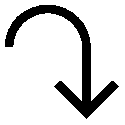
\includegraphics[height=12pt]{editor-toolbar-redo} (redo), the user can undo or redo actions he/she made in the drawing area. This actions are also available as keyboard shortcuts: \textsf{Ctrl-Z} or \textsf{Ctrl-Y}, respectively.

\subsubsection{Clipboard (Copy \& Paste)}

The editor includes a clipboard. It is possible to transfer selected cells using the 
\includegraphics[height=12pt]{editor-toolbar-clone}
 button (copy) or the keyboard shortcut \textsf{Ctrl-C} to the clipboard.
The contents of the clipboard can then be pasted by using the 
\includegraphics[height=12pt]{editor-toolbar-clipboard} button (paste) or the keyboard shortcut \textsf{Ctrl-V}

\subsubsection{Delete}

Selected cells can be removed by clicking the \includegraphics[height=12pt]{editor-toolbar-trash} button (delete). Alternatively, this can be done with the keyboard shortcut \textsf{Backspace}.

\subsubsection{Validation}

The action behind the "Validate" button validates the constraints described in \ref{sec:impl-frontend-graphvalidation} for each cell in the drawing area. Invalid cells will be marked with a yellow icon. An additional error message is shown in the tooltip when hovering over that icon.

\begin{figure}
\centering
\begin{subfigure}{.4\textwidth}
  \centering
  \includegraphics[width=.8\linewidth]{validate1}
  \caption{validation errors indicator}
\end{subfigure}
\begin{subfigure}{.4\textwidth}
  \centering
  \includegraphics[width=.8\linewidth]{validate2}
  \caption{validation failed while connecting}
\end{subfigure}
\caption{graph validation}
\label{fig:cell-validation}
\end{figure}

\subsubsection{Load \& Save}

Workflows created by AFCL ToolKit (XML) or even existing AFCL workflows (YAML/JSON) can be loaded in order to visualize or doing further editing. To load a workflow, the user can click on the "Load" button in the toolbar and choose the desired file in the dialog.

To save a workflow, the user can click on the "Save" button in the toolbar.
This results in a download offered by the tool. The user can then choose the target location.  When saving a workflow, the desired format can be selected out of XML, JSON or YAML.\\
With XML, additional graphical information is stored among the serialized workflow, what means that the workflow will be exactly in the same state when opened later.\\
JSON an YAML deliver an AFCL compliant workflow.

\section{Settings}

The purpose of the Settings component is to provide an interface to view and adjust application-wide constants. 


\chapter{Evaluation}

This section evaluates AFCL ToolKit and compares the effort for creating and adapting AFCL workflows using the tool with the effort needed to write or adapt the AFCL workflow manually in a text file or using the Java API.

The \textit{Gate Change Alert}  (GCA), and \textit{Anomaly Detection} (AD) and \textit{Genome} (GEN) AFCL workflow examples from \citep{online-afcl-dps} are used as evaluation models.

It has to be noted, that only the time it took to get the final result - which is an AFCL workflow in a YAML file - is evaluated.
The learning time to understand the AFCL function choreography system, the Java API or to become familiar with AFCL Toolkit is not considered in this study.

\section{Methodology}

In this section, the methodology for the evaluations in sections \ref{sec:evaluation-composing} and \ref{sec:evaluation-adapting} is explained:

One computer science student learned the workflow language AFCL, its Java-based API and knows how to use AFCL ToolKit.
Then the different workflows are composed (section \ref{sec:evaluation-composing} or adapted (section \ref{sec:evaluation-adapting}) by
\begin{enumerate}[label={(\arabic*)}]
	\item editing the text file manually (writing YAML by hand),
	\item using the AFCL Java API,
	\item using AFCL ToolKit.
\end{enumerate}

The results are then compared to each other.

\section{Composing Workflows}
\label{sec:evaluation-composing}

In this section, the development effort of the three example workflows is measured, using the three introduced methods.

It took approximately 55 minutes to compose the GCA workflow with method (1), approximately 25 minutes with method (2) and approximately 22 minutes with method (3).\\
For the AD workflow it took approximately 75 minutes with method (1), approximately 42 minutes with method (2) and approximately 37 minutes with method (3).\\
The GEN workflow took approximately 49 minutes with method (1), approximately 24 minutes with method (2) and approximately 20 minutes with method (3).

Figure \ref{fig:evaluation-composing} shows a visualization of the evaluation.

\begin{figure}[h]
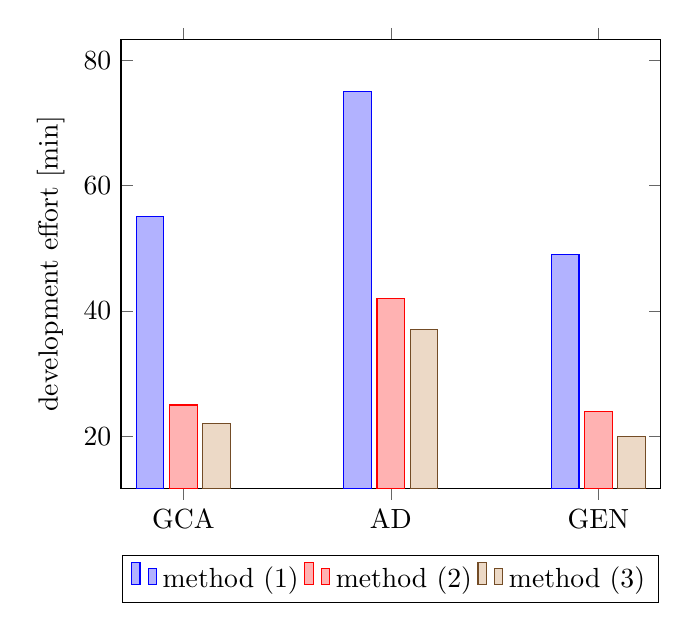
\begin{tikzpicture}
\begin{axis}[
    ybar,
    enlargelimits=0.15,
    legend style={at={(0.5,-0.15)},
      anchor=north,legend columns=-1},
    ylabel={development effort [min]},
    symbolic x coords={GCA,AD,GEN},
    xtick=data,
    nodes near coords align={vertical},
    ]
\addplot coordinates {(GCA,55) (AD,75) (GEN,49)};
\addplot coordinates {(GCA,25) (AD,42) (GEN,24)};
\addplot coordinates {(GCA,22) (AD,37) (GEN,20)};
\legend{method (1),method (2),method (3)}
\end{axis}
\end{tikzpicture}
\caption{Evaluated development effort for creating GCA, AD and GEN AFCL workflows using different methods.\\ \small{method (1): edit text file manually, method (2): AFCL Java API, method (3): AFCL ToolKit}}
\label{fig:evaluation-composing}
\end{figure}

% toolkit has to insert functions first
% java has to set up a project with AFCL API JAR
This evaluation shows, that using AFCL ToolKit can speed up the process for creating AFCL workflows significantly.\\
A big benefit of using AFCL ToolKit over using the Java API is, that anyone with knowledge about AFCL could create the workflow, there is no need to be a programmer.\\
Additionally, human errors are minimized. According to \cite{books-code-complete-mcconnell} the error rate of a developer is between 1.5\% and 5\% in average.
With AFCL ToolKits' immediate validation while creating a workflow, such errors are minimized further. 

\section{Adapting Workflows}
\label{sec:evaluation-adapting}

In this section, the effort for doing a workflow adaptation as described in \ref{sec:backend-adaptation} is measured.

For this evaluation, it is sufficient only measure the effort needed to divide a loop manually into two loops. Since the procedure would be the same for every additional loop, the total approximated effort can then be determined by multiplying the effort which was needed for a divide into two loops, with the number of divides.
In the following, we will only consider the GCA workflow example, since this includes one \texttt{ParallelFor} loop.
The effort is also dependent of the number of affected data elements in the subsequent functions, which have to be adjusted. In the GCA workflow, there are twelve data elements which needs update after a divide.

To divide the loop of the GCA workflow into two loops, it took approximately 27 minutes using method (1), approximately 19 minutes using method (2) and 1 minute using method (3).

\begin{figure}[h]
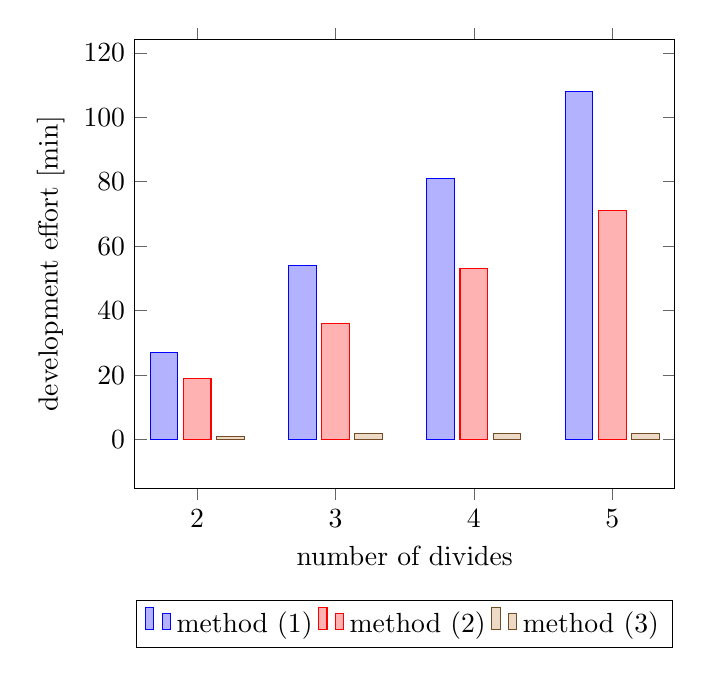
\begin{tikzpicture}
\begin{axis}[
    ybar,
    enlargelimits=0.15,
    legend style={at={(0.5,-0.25)},
      anchor=north,legend columns=-1},
    ylabel={development effort [min]},
    xlabel={number of divides},
    xtick=data,
    nodes near coords align={vertical},
    ]
\addplot coordinates {(2,27) (3,54) (4,81) (5,108)};
\addplot coordinates {(2,19) (3,36) (4,53) (5,71)};
\addplot coordinates {(2,1) (3,2) (4,2) (5,2)};
\legend{method (1),method (2),method (3)}
\end{axis}
\end{tikzpicture}
\caption{Evaluated development effort for adapting workflows using different methods.\\ \small{method (1): edit text file manually, method (2): AFCL Java API, method (3): AFCL ToolKit}}
\label{fig:evaluation-adaptation}
\end{figure}

% benefit for backend
% split parallel loops to n loops
% realistic example
% company average uses five clouds (paper/website ?)
% how much time would be needed to update manually
% maybe twenty gates will change for a bigger airport
% run multiple workflows each with big number of passengers
% with system update automatically workflows

% Related work (optional)?

\chapter{Conclusion}

With AFCL ToolKit, a system was developed that greatly simplifies the creation and adaptation of AFCL workflows. 
The implemented system fulfills the requirement of modeling workflows at a high level of abstraction by providing an editor where workflows can be created and edited in a WYSIWYG manner. It even goes further by providing additional user actions like clipboard, versioning, auto-layout and validation, which make the creation process more convenient.
The system also can load existing AFCL workflows for visualization and further editing and supports three different formats for exporting workflows.

We have shown that the system with its benefits leads to an enormous speed up for workflow development and adaption.
With these possibilities, AFCL is no longer reserved exclusively for developers. By using this tool, technically anyone is able to develop a workflow.

\section{Future Work}

\begin{itemize}
	\item additional information in tooltips
	\item auto-complete for \texttt{source} fields
	\item visualize data flow
\end{itemize}

\begin{appendix}


\chapter{AFCL API functions}
\label{apx:afcl-functions}

In the following paragraphs of this section, terms highlighted with a mono-spaced font refer to classes or class properties of the AFCL Java API.

The AFCL Java API in its current state provides classes which define function and control-structure objects, as well as data-flow objects of an AFCL workflow. They can be arranged and nested in a tree structure in order to model the execution flow.

However, the API has its limitations. One is that a \texttt{Function} does not have a reference to its \textit{parent object}. The \textit{parent object} can be either a \texttt{Workflow} or \texttt{Compound}, which has its own implementation to access its enclosed functions - there is no common super class or interface providing a common method. The same problem occurs on \texttt{DataIns}, \texttt{DataOuts} and \texttt{DataOutsAtomic}, they do have properties (e.g. \texttt{source}) in common, but each of them has its own implementation to access them. This is also the case for \texttt{AtomicFunction} and \texttt{Compound} and the \texttt{dataIns} property.\\
Furthermore, tasks like iterating over all \texttt{Function} objects in a \texttt{Workflow} are not supported. 

These limitations make it challenging to perform automated modifications while keep the code generic.
During development, it turned out that the following tasks were required frequently while modifying a workflow programmatically. We define these task  as \textit{general adaptation tasks}:
\begin{itemize}
	\item get a \texttt{Function} by its name
	\item get the \textit{parent object} of a Function (\texttt{Workflow} or \texttt{Compound})
	\item get the \texttt{List} which contains a given \texttt{Function}
	\item get all \texttt{DataIns} and \texttt{DataOuts} which use a given \texttt{Function} as source
	\item traverse a \texttt{Workflow}, in particular, iterate over all \texttt{Function} objects inside a \texttt{Workflow}
\end{itemize}

The generic requirement was achieved one the one hand by using \textit{Reflection}, on the other hand by developing a generic \textit{traverse function}, shown in listings \ref{lst:traverseWorkflow} and \ref{lst:traverseFunctions}.

\begin{lstlisting}[language=Java,caption={Traverse workflow},label={lst:traverseWorkflow}]
public static void traverseWorkflow(Workflow wf, BiConsumer<Function, Object> consumer) {
    traverseFunctions(wf.getWorkflowBody(), consumer, wf);
}
\end{lstlisting}

\begin{lstlisting}[language=Java,caption={Traverse functions},label={lst:traverseFunctions}]
public static void traverseFunctions(List<Function> functionsList, BiConsumer<Function, Object> consumer, Object currentParent) {
    if (functionsList == null) {
        return;
    }
    for (Function fn : functionsList) {
        consumer.accept(fn, currentParent);
        if (fn instanceof IfThenElse) {
            traverseFunctions(((IfThenElse) fn).getThen(), consumer, fn);
            traverseFunctions(((IfThenElse) fn).getElse(), consumer, fn);
        }
        if (fn instanceof Switch) {
            for (Case c : ((Switch) fn).getCases()) {
                traverseFunctions(c.getFunctions(), consumer, fn);
            }
        }
        if (fn instanceof Parallel) {
            for (Section s : ((Parallel) fn).getParallelBody()) {
                traverseFunctions(s.getSection(), consumer, fn);
            }
        }
        if (fn instanceof ParallelFor) {
            traverseFunctions(((ParallelFor) fn).getLoopBody(), consumer, fn);
        }
    }
}
\end{lstlisting}

As the reader may have noticed, the traverse function accepts Java's \texttt{BiConsumer} as second argument, which makes it very versatile in its usage. The given consumer operation - which can be a function reference or a lambda expression - is executed for every function element in the workflow, providing the element itself and its \textit{parent object} as arguments on traversal. This is indeed very powerful, reduces LOC, therefore improves readability, maintainability and efficiency. The only drawback is that all functions are always visited, because there is no proper way to break out of a lambda expression. There exist approaches to break out by throwing an Exception, however this is considered to be bad practice.

For example, getting a function by its name, can be achieved as showed in listing \ref{lst:getFuncByName}. \small Note that mutating variables in lamda expressions is not thread-safe, so an \texttt{AtomicReference} is used.

\begin{lstlisting}[language=Java,caption={get a function by its name},label=lst:getFuncByName]
final AtomicReference<Function> fRef = new AtomicReference<>();
traverseFunctions(fnList, (fn, parentObj) -> {
    if (fn.getName() != null && fn.getName().equals(name)) {
        fRef.set(fn);
    }
});
// do something with found function in fRef.get();
\end{lstlisting}

\end{appendix}

\printbibliography

\end{document}
